\section{Method}
\label{sect:method}
In this section, we describe an unsupervised method for TF design. Our method generates a semi-automated material classification and an initial TF specification. These elements are still combined to produce a simplified design interface and an intuitive volume exploration space. 

Fig.~\ref{fig:volume-exploration-pipeline} shows an overview of the proposed method. In a pre-processing step, the dataset is organized into a regular volume grid. Given that the input data is unlabeled, all techniques are applied from an unsupervised perspective. 

\begin{figure*}[htb!]
    \centering
    \caption{Overview of the proposed unsupervised method for transfer function definition and design.}
    \label{fig:volume-exploration-pipeline}
    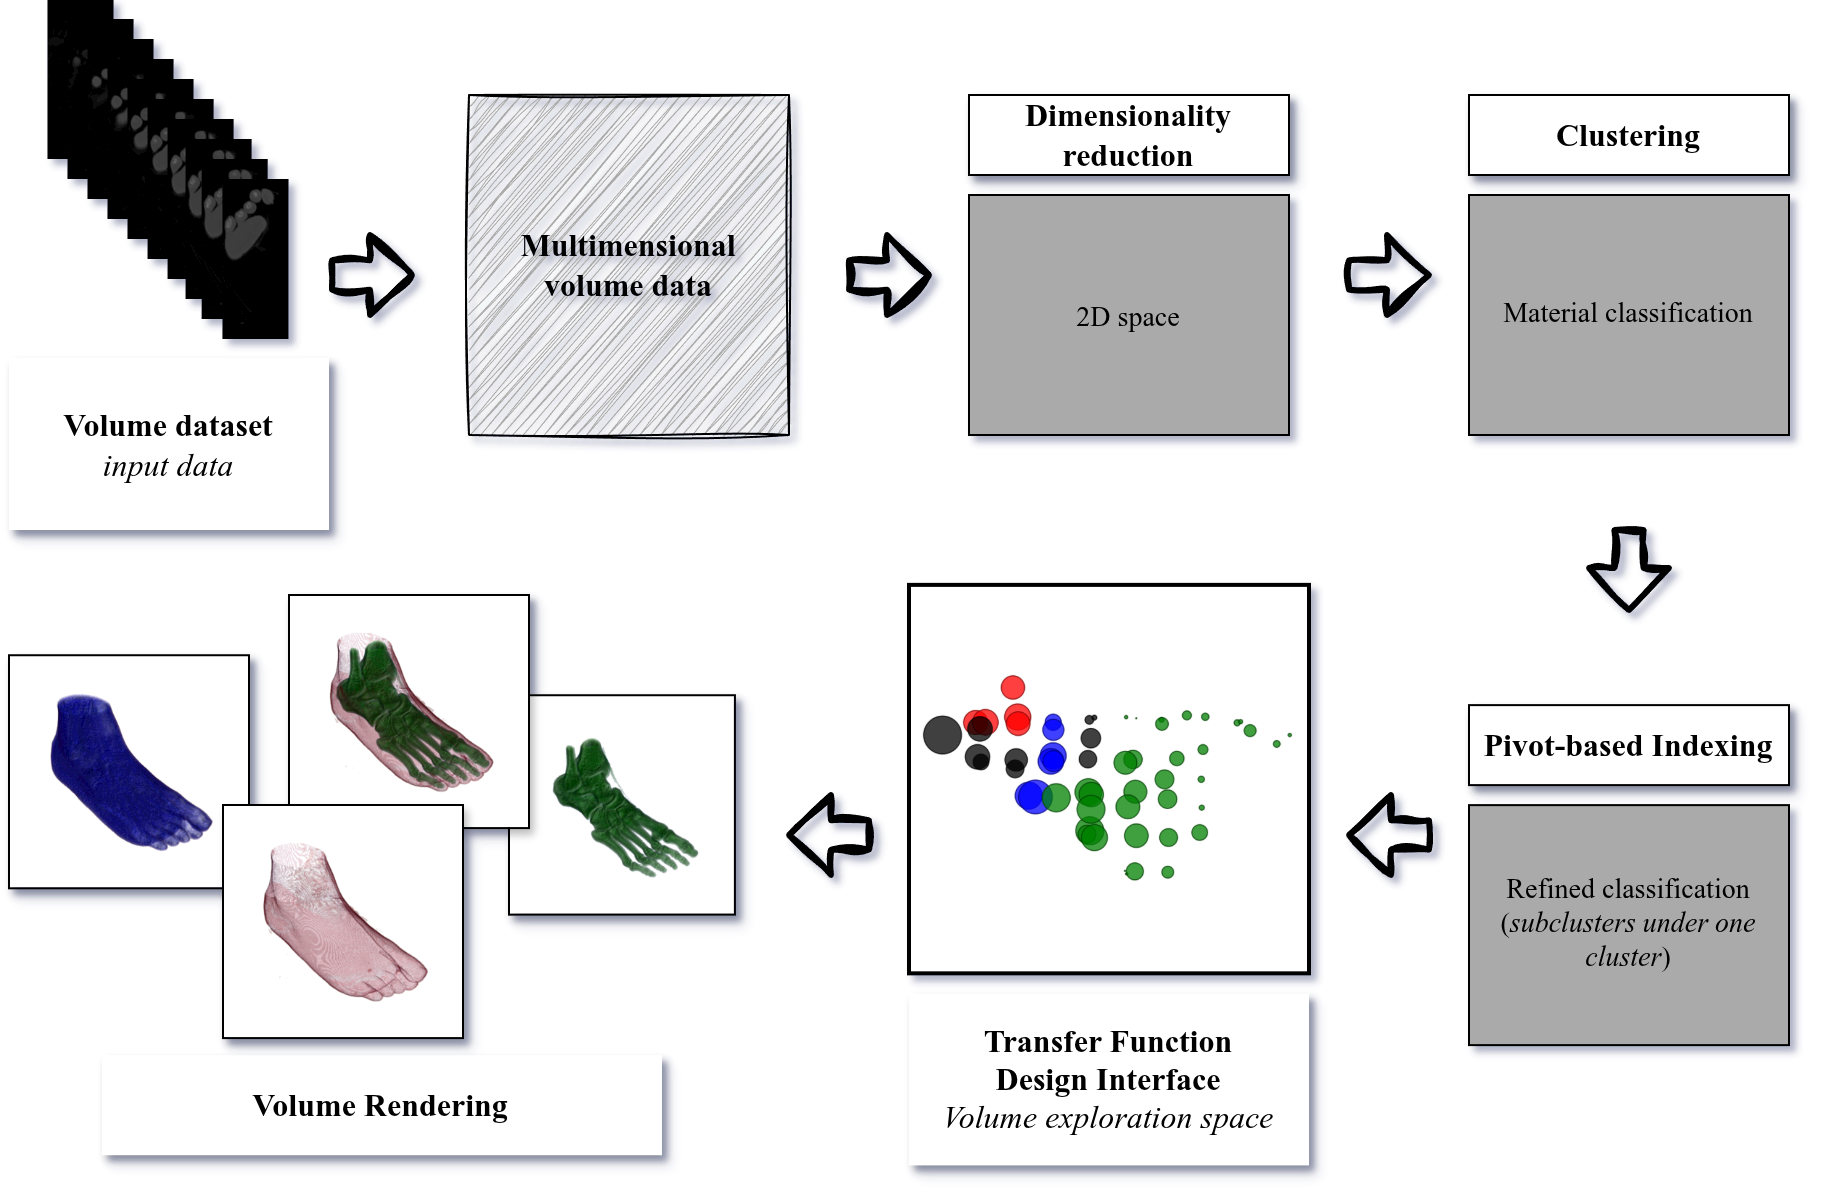
\includegraphics[width=\textwidth]{figs/method-overview.png}
\end{figure*}



\subsection{Dimensionality Reduction}
\label{subsect:feature-extraction}
The first step of our method is a dimensionality reduction. It serves two primary purposes. Firstly, it structures a 2D interface for the TF design and the volume exploration space. Secondly, it prepares the data for the clustering step, which requires 2D input.

We employed a feature extraction technique in this step. Besides the dimensionality reduction, it minimizes information loss once the feature selection step removes irrelevant and redundant attributes.

FastMap~\cite{faloutsos1995}, a classical MDS algorithm, is the feature extraction technique used. We take into account the three advantages of applying this technique: low time complexity cost even with large datasets~\cite{faloutsos1995}, flexibility to handle high-dimensional datasets~\cite{faloutsos1995}, and ability to preserve the clustering structure of the original data~\cite{fodor2002, khan2014}. Another advantage is that no input parameter is required. The time complexity of the FastMap algorithm is $\mathcal{O} (nk)$, where $n$ is the total number of voxels and $k$, is the dimensionality of the target space.

Let $d$ be the original dimensionality of input data, the algorithm projects $n$ samples into a $k$-dimensional space, where $k <= d$. Here, $n$ is the total number of voxels, $d$ is the number of original attributes (dimensionality) and $k = 2$. FastMap is a recursive algorithm that can be succinctly described in the following steps:
\begin{enumerate}
    \item Find the two points, named as pivots, furthest away from each other in a dataset.
    \item Project the remaining points onto a hyperplane orthogonally positioned between the pivots.
\end{enumerate} 

Strategies capable of precisely identifying pivots have at least quadratic time complexity. To avoid compromising runtime, \cite{faloutsos1995} developed a heuristic that is presented in Algorithm~\ref{alg:pivot-searching-of-fastmap}. It takes a set of points $\mathbb{O}$ and  approximately finds the pair of points $O_a$ and $O_b$ that are the farthest from each other. In our approach, each point is a voxel, and thus, $\mathbb{O}$ is the set of all voxels. The algorithm considers only the values of selected attributes.  A voxel's 3D position ($x$, $y$ and $z$) is not used in any calculation.

\begin{algorithm}
    \caption{Pivot searching of FastMap.}
    \label{alg:pivot-searching-of-fastmap}
        \KwIn{$\mathbb{O}$}
        \KwOut{Pivots $O_a$, $O_b$}
        $O_a \gets$ random point $o$ $\in$ $\mathbb{O}$  \\
        $O_b \gets$ point $o$ $\in$ $\mathbb{O}$ farthest from $O_a$\\
        $O_a \gets$ point $o$ $\in$ $\mathbb{O}$ farthest from $O_b$
\end{algorithm}



\subsection{Clustering}
\label{subsect:clustering}
A major goal of our method is to simplify material classification and facilitate the highlighting of volume details. We address this objective by employing a classical density-based clustering algorithm, the DBSCAN~\cite{ester1996}. 

DBSCAN is a widely utilized algorithm known for its success across various applications~\cite{schubert2017}. Nevertheless, its adoption in DVR comes with some caveats.  The original version~\cite{ester1996} exhibits a time complexity of $\mathcal{O} (n^2)$ in the worst case~\cite{schubert2017}. With practical usability in mind, we implemented a grid-based  DBSCAN proposed by \cite{gunawan2013}. This version claims a time complexity of $\mathcal{O} (n \log (n))$. 

Like the original algorithm~\cite{ester1996}, the 2D grid version also has $minPts$ and $\varepsilon$ as input parameters. In this way, the user must fine-tune such parameters to best classify the volume data. 

When this method step ends, each cluster comprises a subset of voxels that potentially represent a region of interest.

\subsubsection{Grid-based DBSCAN of \cite{gunawan2013}} 

\cite{gunawan2013} introduces the concept of a grid to improve the efficiency of the clustering process, especially for high-dimensional datasets. The authors improve the scalability and efficiency of traditional DBSCAN by leveraging grid-based partitioning and density estimation techniques. Detailed explanations are provided in the works of \cite{gunawan2013} and \cite{gan2015}. The algorithm operates on a cell grid and comprises the tasks summarized next.

\begin{enumerate}
    \item Grid partitioning. The first step involves partitioning the space into a grid of cells. Each cell represents a small portion of the entire space.

    \item Density estimation. Within each cell, the algorithm calculates the density of points. The density is usually estimated using a distance threshold ($\varepsilon$) to determine the neighborhood of each point.

    \item Identifying core points. Points with a density above a certain threshold ($minPts$) are considered core points. These core points are potential seeds for clusters.

    \item Expanding clusters. Starting from a core point, the algorithm expands the cluster by iteratively adding neighboring points that also qualify as core points. The expansion continues until there are no more core points to be added.

    \item Handling border points. Points that are within the $\varepsilon$ neighborhood of a core point but do not meet the density requirement to be considered core themselves are classified as border points. Border points are assigned to the cluster of their nearest core point.

    \item Handling noise. The points that are not core and do not belong to any cluster are considered noise points.
\end{enumerate}

\subsection{Pivot-based indexing}
\label{subsect:pivot-based-indexing}

Our TF design interface revolves around a scatter plot view. Attempting to plot the entire dataset is impractical due to the high cognitive load and computational cost involved. To overcome this challenge, we implement a pivot-based indexing approach within each cluster identified by DBSCAN. Only the pivots within each cluster are plotted, thereby reducing visual density.

This step also serves as a second-level clustering process, refining each classified volume detail. Once the pivots are identified, each point in a cluster is assigned to the nearest pivot, as outlined in Algorithm~\ref{alg:subclustering-finding}. Therefore, a cluster is divided into sub-clusters represented by pivots.

Let $\mathbb{P}$ denote the set of all points within a cluster $c$, and $\mathbb{P}_s$ represent the selected pivots of the same cluster, every point $p \in \mathbb{P}$ is assigned to the sub-cluster of the nearest pivot $p_s \in \mathbb{P}_s$.

\begin{algorithm}
    \caption{Finding sub-clusters within a cluster.}
    \label{alg:subclustering-finding}
        \KwIn{Set of points $\mathbb{P}$ of a cluster $c$}
        \KwIn{Set of pivots $\mathbb{P}_s$ of a cluster $c$}
        \KwOut{Set of points $\mathbb{P}$ with associated sub-clusters}
        \ForEach{$p \in \mathbb{P}$}{
            $p_s \gets$ $p$ nearest pivot in $\mathbb{P}_s$  \\
            $p$ assigned to $p_s$'s sub-cluster 
        }
\end{algorithm}

\subsubsection{Sparse Spatial Selection}

We use the Sparse Spatial Selection (SSS) for pivot-based indexing. This algorithm~\cite{pedreira2007} is known for its straightforward implementation and low computational cost compared to other pivot-based techniques. 

An overview of the SSS is shown in Algorithm~\ref{alg:sss}. It identifies the points furthest from each other, termed pivots. Let $\mathbb{P}$ be a set of points, $alpha$ a distance factor within the interval $[0, 1]$, the first point $p_1 \in \mathbb{P}$ is added to the pivots $\mathbb{P}_s$. Subsequently, the algorithm traverses $\mathbb{P}$ to find additional pivots. With $M$ representing the maximum distance between two arbitrary points, a point $p$ is added to the pivots $\mathbb{P}_s$ only if $\forall p_s \in \mathbb{P}_s$, $\verb|dist|(p, p_s) \geq M\alpha$, where \verb|dist| is a distance function and $p_s$ is a pivot $ \in \mathbb{P}_s$.


\begin{algorithm}
    \caption{Sparse Spatial Selection.}
    \label{alg:sss}
        \KwIn{Set of points $\mathbb{P}$}
        \KwOut{Set of selected pivots $\mathbb{P}_s$}
        $\mathbb{P}_s \gets {p_1}$\\
        \ForEach{$p \in \mathbb{P}$}{
            \If{$\forall p_s \in \mathbb{P}_s$, dist$(p, p_s) \geq M\alpha$}{     
                $\mathbb{P}_s \gets \mathbb{P}_s \cup \{p\} $
            }
        }
\end{algorithm}

To control the number of pivots, users can adjust the distance factor $\alpha$. A smaller $\alpha$ value favours selecting a greater number of pivots, while a value closer to $1$ results in fewer pivots.